\subsection{Durchführung}
\label{sec:durchführung}
Bevor die eigentliche Durchführung der Versuchsteile beginnt, wird die Heizspannung für das Reflexklystron ca. 10 Minuten vor Versuchsbeginn eingestellt.

\subsubsection{Durchführung des ersten Versuchsteils}
Der Versuch wird wie in Abbildung \ref{sec:aufbau1} beschrieben aufgebaut.
Das Dämpfungsglied wird auf den passenden Wert für $\SI{30}{\decibel}$ eingestellt.
Die Reflektorspannung wird auf Wechselspannung gestellt und auf die x-Achse des Oszillographen gegeben, während das Signal des Detektors auf die y-Achse gegeben wird.
Hierdurch ergibt sich eine Kurve, die wie in Abbildung \ref{fig:output} dargestellt, eine Mode repräsentiert.

\begin{figure}
  \centering
  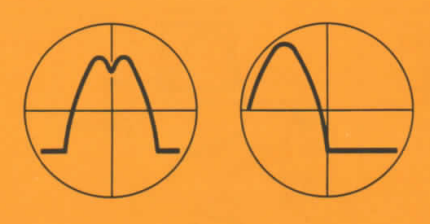
\includegraphics[height=5cm]{ressources/df1.png}
  \caption{Beobachtete Bodenkurve \cite{skript}. Links der durch den Frequenzmesser verursachte "Dip". Rechts die Messung der unteren Reflektorspannung. }
  \label{fig:df1}
\end{figure}

Die Reflektorspannung wird so gewählt, dass die Mitte der Mode mittig auf der x-Achse des Oszillographen liegt.
Zusätzlich wird die Mittenfrequenz bestimmt, indem der Frequenzmesser zu eingestellt wird, dass ein "Dip" in der Mitte der Mode zu sehen ist, wie es links in Abbildung \ref{fig:df1} dargestellt ist.
Die Mittenfrequenz, die passende Reflektorspannung sowie die Amplitude der Mode werden notiert.
Außerdem wird, wie in Abbildung \ref{fig:df1} rechts dargestellt, die untere sowie auch die obere Spannungsansatz-Spannung gemessen.
Dazu wird die Reflektorspannung so gewählt, dass sich ebendieses Bild ergibt.

Der gesamte Messvorgang wird für zwei weitere Moden wiederholt, welche in anderen Bereichen der Resonatorspannung zu finden sind.

Als weiterer Messprozess werden die Punkte der höchsten Mode gemessen, welche der vollen bzw. der halben Signalleistung entsprechen.
Hierzu wird die Mode über die Reflektorspannung vertikal jeweils auf die Mitte der Mode, den linken Punkt der mittleren Leistung bzw. auf den rechten Punkt der mittleren Leistung zentriert.
Die Frequenzen werden wiederum über den Frequenzmesser und den im Oszillographen beobachtbaren "Dip" ermittelt.
Die Reflektorspannungen sowie die Freuqenzen für die drei Punkte weden notiert.

\subsubsection{Durchführung des zweiten Versuchsteils}

Der Versuch wird wie in Abbildung \ref{sec:aufbau2} beschrieben aufgebaut, wobei zunächst der Abschluss eingebaut wird.

Das Reflexklystron wird mit einer Rechteck-Spannung moduliert Dämpfungsglied sowie Einstellung des SWR-Meters so gewählt, dass ein maximaler Ausschlag am SWR-Meter innerhalb des Skalenbereiches zu beobachten ist.
Es wird die im vorherigen Versuchsteil gefundene Mittenfrequenz der höchsten Mode verwendet.

Es wird nun der Abschluss durch den Kurzschluss ersetzt.
Mithilfe des Stehwellen-Detektors werden zwei Punkte minimalen Ausschlages am SWR-Meter gesucht und dessen Position notiert.

Zuletzt wird eine Dämpfungskurve aufgenommen, wozu der Kurzschluss am Hohlleiter wieder durch einen Abschluss ersetzt wird.
Das SWR-Meter wird so eingestellt, dass es bei einer vorgegebenen Einstellung durch das Dämpfungsglied einen maximalen Ausschlag von $\SI{0}{\decibel}$ anzeigt.
Die Dämpfung wird nun verstärkt, bis jeweils ein Ausschlag von $\SI{2}{\decibel}, \SI{4}{\decibel}, \SI{6}{\decibel}, \SI{8}{\decibel}, \SI{10}{\decibel}$ am SWR-Meter abzulesen ist.
Die Einstellungen des Dämpfungsgliedes an diesen Punkten werden notiert.

\subsubsection{Durchführung des dritten Versuchsteils}

Der Versuch wird wie in Kapitel \ref{sec:aufbau3} beschrieben aufgebaut.
Das Reflexklystron bleibt bei der im vorherigen Versuchsteil gewählten Einstellung.
Es sollen die Stehwellenverhältnissen mit den in Kapitel \ref{sec:steh} umschriebenen Methoden bestimmt werden.

Die erste Methode wird für die Einstellungen des Gleitschraubentransformators von $\SI{3}{\milli\metre}$, $\SI{5}{\milli\metre}$ und $\SI{7}{\milli\metre}$ durchgeführt.
Der Stehwellendetektor wird so platziert, dass das SWR-Meter ein maximales Signal detektiert.
Dieses Signal wird durch die Einstellung des SWR-Meters auf $\num{1.0}$ normiert.
Daraufhin wird die Sonde in ein Minimum verschoben und der Wert des SWR-Meters dort gemessen.

Bei der zweiten Methode, der "3 dB-Methode", wird der Gleitschraubentransformator auf $\SI{9}{\milli\metre}$ eingestellt, was einem höheren Stehwellenverhältnis entspricht.
Die Messsonde wird vertikal bewegt, bis sich ein Minimum am SWR-Meter ergibt.
Dieses wird auf einen Wert von $\SI{3}{\decibel}$ normiert.
Die Sonde wird nun einmal nach rechts und einmal nach links bewegt, bis sich ein Wert von $\SI{0}{\decibel}$ auf dem SWR-Meter ergibt.
Diese Werte werden notiert.

Zum Schluss wird die "Abschäwcher-Methode" genutzt, wobei auch hier der Gleitschraubentransformator auf $\SI{9}{\milli\metre}$ eingestellt wird.
Wiederum wird die Sonde vertikal bewegt, bis das SWR-Meter ein Minimum anzeigt.
Darufhin wird das Dämpfungsglied auf $\SI{20}{\decibel}$ eingestellt und die Einstellungen am SWR-Meter so gewählt, dass dort ein Wert von $\SI{3}{\decibel}$ angezeigt wird.
Die Sonde wird nun vertikal bewegt, bis das Signal ein relatives Maximum anzeigt.
Das Dämpfungsglied wird an dieser Stelle so verstellt, dass das SWR-Meter wieder $\SI{3}{\decibel}$ anzeigt.
Die Dämpfungsgliedeinstellung wird notiert.
